\documentclass[journal,12pt,twocolumn]{IEEEtran}
\usepackage{setspace}
\usepackage{gensymb}
\usepackage{xcolor}
\usepackage{caption}
\singlespacing
\usepackage{siunitx}
\usepackage[cmex10]{amsmath}
\usepackage{mathtools}
\usepackage{hyperref}
\usepackage{amsthm}
\usepackage{mathrsfs}
\usepackage{txfonts}
\usepackage{stfloats}
\usepackage{cite}
\usepackage{cases}
\usepackage{subfig}
\usepackage{longtable}
\usepackage{multirow}
\usepackage{enumitem}
\usepackage{bm}
\usepackage{mathtools}
\usepackage{listings}
\usepackage{tikz}
\usetikzlibrary{shapes,arrows,positioning}
\usepackage{circuitikz}
\renewcommand{\vec}[1]{\boldsymbol{\mathbf{#1}}}
\DeclareMathOperator*{\Res}{Res}
\renewcommand\thesection{\arabic{section}}
\renewcommand\thesubsection{\thesection.\arabic{subsection}}
\renewcommand\thesubsubsection{\thesubsection.\arabic{subsubsection}}

\renewcommand\thesectiondis{\arabic{section}}
\renewcommand\thesubsectiondis{\thesectiondis.\arabic{subsection}}
\renewcommand\thesubsubsectiondis{\thesubsectiondis.\arabic{subsubsection}}
\hyphenation{op-tical net-works semi-conduc-tor}

\lstset{
language=Python,
frame=single, 
breaklines=true,
columns=fullflexible
}
\begin{document}
\theoremstyle{definition}
\newtheorem{theorem}{Theorem}[section]
\newtheorem{problem}{Problem}
\newtheorem{proposition}{Proposition}[section]
\newtheorem{lemma}{Lemma}[section]
\newtheorem{corollary}[theorem]{Corollary}
\newtheorem{example}{Example}[section]
\newtheorem{definition}{Definition}[section]
\newcommand{\BEQA}{\begin{eqnarray}}
\newcommand{\EEQA}{\end{eqnarray}}
\newcommand{\define}{\stackrel{\triangle}{=}}
\newcommand{\myvec}[1]{\ensuremath{\begin{pmatrix}#1\end{pmatrix}}}
\newcommand{\mydet}[1]{\ensuremath{\begin{vmatrix}#1\end{vmatrix}}}
\bibliographystyle{IEEEtran}
\providecommand{\nCr}[2]{\,^{#1}C_{#2}} % nCr
\providecommand{\nPr}[2]{\,^{#1}P_{#2}} % nPr
\providecommand{\mbf}{\mathbf}
\providecommand{\pr}[1]{\ensuremath{\Pr\left(#1\right)}}
\providecommand{\qfunc}[1]{\ensuremath{Q\left(#1\right)}}
\providecommand{\sbrak}[1]{\ensuremath{{}\left[#1\right]}}
\providecommand{\lsbrak}[1]{\ensuremath{{}\left[#1\right.}}
\providecommand{\rsbrak}[1]{\ensuremath{{}\left.#1\right]}}
\providecommand{\brak}[1]{\ensuremath{\left(#1\right)}}
\providecommand{\lbrak}[1]{\ensuremath{\left(#1\right.}}
\providecommand{\rbrak}[1]{\ensuremath{\left.#1\right)}}
\providecommand{\cbrak}[1]{\ensuremath{\left\{#1\right\}}}
\providecommand{\lcbrak}[1]{\ensuremath{\left\{#1\right.}}
\providecommand{\rcbrak}[1]{\ensuremath{\left.#1\right\}}}
\theoremstyle{remark}
\newtheorem{rem}{Remark}
\newcommand{\sgn}{\mathop{\mathrm{sgn}}}
\newcommand{\rect}{\mathop{\mathrm{rect}}}
\newcommand{\sinc}{\mathop{\mathrm{sinc}}}
\providecommand{\abs}[1]{\left\vert#1\right\vert}
\providecommand{\res}[1]{\Res\displaylimits_{#1}} 
\providecommand{\norm}[1]{\lVert#1\rVert}
\providecommand{\mtx}[1]{\mathbf{#1}}
\providecommand{\mean}[1]{E\left[ #1 \right]}
\providecommand{\fourier}{\overset{\mathcal{F}}{ \rightleftharpoons}}
\providecommand{\ztrans}{\overset{\mathcal{Z}}{ \rightleftharpoons}}
\providecommand{\system}[1]{\overset{\mathcal{#1}}{ \longleftrightarrow}}
\newcommand{\solution}{\noindent \textbf{Solution: }}
\providecommand{\dec}[2]{\ensuremath{\overset{#1}{\underset{#2}{\gtrless}}}}
\let\StandardTheFigure\thefigure
\def\putbox#1#2#3{\makebox[0in][l]{\makebox[#1][l]{}\raisebox{\baselineskip}[0in][0in]{\raisebox{#2}[0in][0in]{#3}}}}
     \def\rightbox#1{\makebox[0in][r]{#1}}
     \def\centbox#1{\makebox[0in]{#1}}
     \def\topbox#1{\raisebox{-\baselineskip}[0in][0in]{#1}}
     \def\midbox#1{\raisebox{-0.5\baselineskip}[0in][0in]{#1}}

\vspace{3cm}
\title{Conic Assignment}
\author{Gautam Singh}
\maketitle
\bigskip

\begin{abstract}
    This document contains the solution to Question 27 of Exercise 5 in Chapter
    6 of the class 12 NCERT textbook.
\end{abstract}

\begin{enumerate}
    \item The point on the curve 
    \begin{align}
        x^2 = 2y
        \label{eq:curve}
    \end{align}
    which is nearest to the point 
    $\vec{P} = \myvec{0\\5}$ is
    \begin{enumerate}
        \item $\myvec{2\sqrt{2}\\4}$
        \item $\myvec{2\sqrt{2}\\0}$
        \item $\myvec{0\\0}$
        \item $\myvec{2\\2}$
    \end{enumerate}

    \solution We rewrite the conic \eqref{eq:curve} in matrix form.
    \begin{align}
        \vec{x}^\top\myvec{1&0\\0&0}\vec{x} + 2\myvec{0&-1}\vec{x} = 0
        \label{eq:curve-mtx}
    \end{align}
    Comparing with the general equation of the conic,
    \begin{align}
        \vec{V} &= \myvec{1&0\\0&0} \label{eq:V-val} \\
        \vec{u} &= \myvec{0\\-1} \label{eq:u-val} \\
        f &= 0 \label{eq:f-val}
    \end{align}
    Therefore, the equation of the normal where $\vec{u}$ is the point of contact 
    and $\vec{R} \triangleq \myvec{0&-1\\1&0}$ is
    \begin{align}
        \brak{\vec{Vq}+\vec{u}}^\top\vec{R}\brak{\myvec{0\\5}-\vec{q}} &= 0
        \label{eq:normal}
    \end{align}
    Substituting the appropriate values and simplifying, we get the equation
    \begin{align}
        \vec{q}^\top\myvec{0&1\\0&0}\vec{q} + 2\vec{q}^\top\myvec{-2\\0} = 0
        \label{eq:q-eqn}
    \end{align}
    Comparing with the general equation of the conic,
    \begin{align}
        \vec{V'} &= \myvec{0&1\\0&0} \label{eq:V-q-val} \\
        \vec{u'} &= \myvec{-2\\0} \label{eq:u-q-val} \\
        f' &= 0 \label{eq:f-q-val}
    \end{align}
    To solve \eqref{eq:q-eqn}, we must make $\vec{V'}$ symmetric. Thus,
    substituting $\vec{V'} \leftarrow \frac{\vec{V'}+\vec{V'}^\top}{2}$,
    the equation becomes
    \begin{align}
        \vec{q}^\top\myvec{0&\frac{1}{2}\\\frac{1}{2}&0}\vec{q} + 2\myvec{-2\\0}\vec{q} = 0
        \label{eq:q-affine}
    \end{align}
    Note that
    \begin{align}
        \vec{V'}\myvec{1\\1} &= \myvec{1\\1} \label{eq:v1} \\
        \vec{V'}\myvec{1\\-1} &= \myvec{-1\\1} \label{eq:v2}
    \end{align}
    and hence the eigenparameters of $\vec{V'}$ are
    \begin{align}
        \vec{P} = \myvec{1&1\\1&-1},\ \vec{D} = \myvec{1&0\\0&-1}
    \end{align}
    Applying the affine transformation and since $\det{V'} = -\frac{1}{4} \neq 0$, 
    \eqref{eq:q-affine} becomes
    \begin{align}
        \vec{y}^\top\vec{Dy} = f_0
        \label{eq:y-affine}
    \end{align}
    where
    \begin{align}
        \vec{q} &= \vec{Py} + \vec{c} \\
        \vec{c} &= -\vec{V'}^{-1}\vec{u} \\
                &= -\myvec{0&1\\1&0}\myvec{-4\\0} = \myvec{0\\4} \\
        f_0 &= \vec{u}^\top\vec{V}^{-1}\vec{u} - f \\
            &= \myvec{-4&0}\myvec{0&1\\1&0}\myvec{-4\\0} = 0
    \end{align}
    Since $f_0 = 0$, we see that \eqref{eq:y-affine} represents a pair of straight lines.
    Expressing $\vec{y} \triangleq \myvec{y_1\\y_2}$, we get
    \begin{align}
        y_1^2-y_2^2 &= 0 \\
        \implies y_1 &= \pm y_2 \\
        \implies \vec{y} &= \myvec{a\\\pm a},\ a \in \mathbb{R}
        \label{eq:y-sol}
    \end{align}
    Hence, using \eqref{eq:y-sol},
    \begin{align}
        \vec{q} &= \vec{Py}+\vec{c} \\
                &= \myvec{a\pm a\\a\mp a+4} \\
        \implies \vec{q} &\in \cbrak{\myvec{2a\\4},\myvec{0\\2a+4}}
        \label{eq:x-case}
    \end{align}
    In the first case, \eqref{eq:curve} implies $a^2 = 2$. In the second case,
    we have $2a + 4 = 0$. Thus, the points of contact are
    \begin{align}
        \vec{N} \in \cbrak{\myvec{\pm 2\sqrt{2}\\4},\myvec{0\\0}}
        \label{eq:poc-ans}
    \end{align}
    The nearest point out of these three candidates for $\vec{N}$ is
    $\myvec{\pm2\sqrt{2}\\4}$. Thus, the correct answer is \textbf{a)}.

    The situation is depicted in Fig. \ref{fig:normal} plotted by the Python
    code \texttt{codes/normal.py}.
    \begin{figure}[!ht]
        \centering
        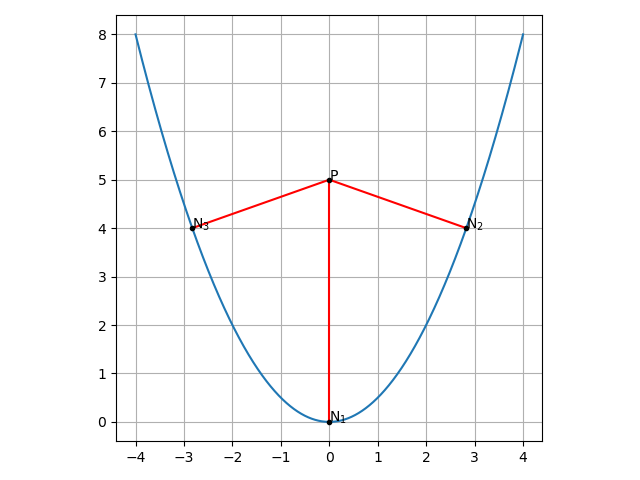
\includegraphics[width=\columnwidth]{figs/normal.png}
        \caption{$N_1,\ N_2,\ N_3$ are the points of contact of the normal from 
        $P$ to the parabola.}
        \label{fig:normal}
    \end{figure}
\end{enumerate}
\end{document}
